\documentclass{sigchi}

% Use this section to set the ACM copyright statement (e.g. for
% preprints).  Consult the conference website for the camera-ready
% copyright statement.

% Copyright
\CopyrightYear{2020}
%\setcopyright{acmcopyright}
\setcopyright{acmlicensed}
%\setcopyright{rightsretained}
%\setcopyright{usgov}
%\setcopyright{usgovmixed}
%\setcopyright{cagov}
%\setcopyright{cagovmixed}
% DOI
\doi{https://doi.org/10.1145/3313831.XXXXXXX}
% ISBN
\isbn{978-1-4503-6708-0/20/04}
%Conference
\conferenceinfo{CHI'20,}{April  25--30, 2020, Honolulu, HI, USA}
%Price
\acmPrice{\$15.00}

% Use this command to override the default ACM copyright statement
% (e.g. for preprints).  Consult the conference website for the
% camera-ready copyright statement.

%% HOW TO OVERRIDE THE DEFAULT COPYRIGHT STRIP --
%% Please note you need to make sure the copy for your specific
%% license is used here!
% \toappear{
% Permission to make digital or hard copies of all or part of this work
% for personal or classroom use is granted without fee provided that
% copies are not made or distributed for profit or commercial advantage
% and that copies bear this notice and the full citation on the first
% page. Copyrights for components of this work owned by others than ACM
% must be honored. Abstracting with credit is permitted. To copy
% otherwise, or republish, to post on servers or to redistribute to
% lists, requires prior specific permission and/or a fee. Request
% permissions from \href{mailto:Permissions@acm.org}{Permissions@acm.org}. \\
% \emph{CHI '16},  May 07--12, 2016, San Jose, CA, USA \\
% ACM xxx-x-xxxx-xxxx-x/xx/xx\ldots \$15.00 \\
% DOI: \url{http://dx.doi.org/xx.xxxx/xxxxxxx.xxxxxxx}
% }

% Arabic page numbers for submission.  Remove this line to eliminate
% page numbers for the camera ready copy
% \pagenumbering{arabic}

% Load basic packages
\usepackage{balance}       % to better equalize the last page
\usepackage{graphics}      % for EPS, load graphicx instead 
\usepackage[T1]{fontenc}   % for umlauts and other diaeresis
\usepackage{txfonts}
\usepackage{mathptmx}
\usepackage[pdflang={en-US},pdftex]{hyperref}
\usepackage{color}
\usepackage{booktabs}
\usepackage{textcomp}
\usepackage{float}
\usepackage{enumitem}
\usepackage{array}
\usepackage{float,wrapfig,subcaption}

% Some optional stuff you might like/need.
\usepackage{microtype}        % Improved Tracking and Kerning
% \usepackage[all]{hypcap}    % Fixes bug in hyperref caption linking
\usepackage{ccicons}          % Cite your images correctly!
% \usepackage[utf8]{inputenc} % for a UTF8 editor only

% If you want to use todo notes, marginpars etc. during creation of
% your draft document, you have to enable the "chi_draft" option for
% the document class. To do this, change the very first line to:
% "\documentclass[chi_draft]{sigchi}". You can then place todo notes
% by using the "\todo{...}"  command. Make sure to disable the draft
% option again before submitting your final document.
\usepackage{todonotes}

% Paper metadata (use plain text, for PDF inclusion and later
% re-using, if desired).  Use \emtpyauthor when submitting for review
% so you remain anonymous.
\def\plaintitle{An evaluation of TRIO’s e-learning module enhancing the communication between cancer patients, clinicians and caregivers}
\def\plainauthor{First Author}
\def\emptyauthor{}
\def\plainkeywords{Usability; user experience; think-alouds; heuristic evaluation; e-learning; medical teaching.}
\def\plaingeneralterms{Documentation, Standardization}

% llt: Define a global style for URLs, rather that the default one
\makeatletter
\def\url@leostyle{%
  \@ifundefined{selectfont}{
    \def\UrlFont{\sf}
  }{
    \def\UrlFont{\small\bf\ttfamily}
  }}
\makeatother
\urlstyle{leo}

% To make various LaTeX processors do the right thing with page size.
\def\pprw{8.5in}
\def\pprh{11in}
\special{papersize=\pprw,\pprh}
\setlength{\paperwidth}{\pprw}
\setlength{\paperheight}{\pprh}
\setlength{\pdfpagewidth}{\pprw}
\setlength{\pdfpageheight}{\pprh}

% Make sure hyperref comes last of your loaded packages, to give it a
% fighting chance of not being over-written, since its job is to
% redefine many LaTeX commands.
\definecolor{linkColor}{RGB}{6,125,233}
\hypersetup{%
  pdftitle={\plaintitle},
% Use \plainauthor for final version.
%  pdfauthor={\plainauthor},
  pdfauthor={\emptyauthor},
  pdfkeywords={\plainkeywords},
  pdfdisplaydoctitle=true, % For Accessibility
  bookmarksnumbered,
  pdfstartview={FitH},
  colorlinks,
  citecolor=black,
  filecolor=black,
  linkcolor=black,
  urlcolor=linkColor,
  breaklinks=true,
  hypertexnames=false
}

% create a shortcut to typeset table headings
% \newcommand\tabhead[1]{\small\textbf{#1}}

% deletes all copyright text on first page:
\makeatletter
\def\@copyrightspace{\relax}
\makeatother

% End of preamble. Here it comes the document.
\begin{document}

\title{\plaintitle}

\numberofauthors{1}
\author{%
  \alignauthor{Melanie Bonnaudet\\
    \affaddr{The University of Sydney}\\
    \affaddr{Sydney, Australia}\\
    \email{melbon@kth.se}}\\
}

\maketitle

\begin{abstract}
 The involvement of carers in oncology is important for the health of cancer diagnosed persons as well as carers themselves. To enhance their involvement in the right direction, three groups; patients, their carers, and clinicians, should maintain good communication. The online platform eTrio has a learning module for each of these three groups, which are based on research from onco-psychologists. This study aims to answer the question; What are the strengths and weaknesses of the TRIO interfaces for clinicians, carers, and patients in terms of their usability? Heuristic evaluation and think-alouds have been conducted to answer this. It has shown that interactive activities as well as neat presented content are engaging the user, buttons and content should have a clear purposes. The TRIO interface will enhance carer’s involvement with a good usability, making it easy for users to retain the important information. Strengths and areas for improvement will be presented in this study. 
\end{abstract}

% Author Keywords
\keywords{\plainkeywords}

\section{Introduction}

Cancer incidences are rising and becoming overall more common, according to Bray. F. et al.’s global cancer statistics 2018 \cite{Bray2018}. As it affects millions of people across the world it is important to provide the best cancer care as possible.

The cancer patient’s medical situation and decisions have impact on its relatives’ life and health \cite{Bevans2012}. Therefore, it is important that relatives can participate in the patient’s medical consultations and decision-making. It has not always been the case that relatives have been allowed to participate [\textbf{reference}]. Each patient should have one main caregiver that can accompany and support the patient. The caregiver and relatives to the patient have expressed needs in medical and behavioural information \cite{Lamore2017}. Oncologists also revealed needs to learn how to provide adapted information for caregivers \cite{Stuij2018}. For an ideal cancer care, patients, caregivers and oncologists need to enhance their communication and behavioural skills for medical situations. 

\textit{"TRIO, Clinician-patient-family working together for quality care"} is a project based on a TRIO Framework, introduced by Laidsaar-Powell, R. et al. \cite{Laidsaar-Powell2017}. It is constituted of three main persons:

\begin{itemize}[noitemsep]
    \item The \textbf{cancer patient}: refers to a cognitively competent adult cancer patient.
    \item The \textbf{main clinician}: usually an oncology physician.
    \item The \textbf{main caregiver}: usually accompanying the patient to medical consultations and assisting in the patient’s care. The caregiver is related to the patient biologically, legally or emotionally.
\end{itemize}

To enhance the communication between cancer patients, their caregivers and oncologists, the TRIO project has created an online learning platform, with content based on TRIO guidelines \cite{Laidsaar-Powell2018a, Laidsaar-Powell2018}. Each group in the TRIO Framework has its own learning platform with learning modules covering different topics. It is a multimedia e-learning platform as it is constituted of text, videos and different interactive activities. These are, for example, yes-no questions, sorting cards according to their importance, surveys about the user’s emotional profile, etc. This type of content makes learning an active process, however inadequate user experience can affect the learning outcome negatively \cite{Huang2005}. Therefore, this study aims to evaluate the usability and use of eTRIO. It investigates the user experience of the TRIO e-learning platform to determine what interactions and presentations of content are needed to successfully meet the users' communication and information needs.

\section{Background}

\subsection{The TRIO Framework and their needs}

Laidsaar-Powell, R. et al. ~\cite{Laidsaar-Powell2017} introduced the notion of a TRIO Framework, also called TRIO Triangle. It is constituted of a cancer patient, a main clinician and a main caregiver. The purpose was to study why it is important to understand the involvement of family caregivers in cancer care. Their study shows to which extent they are involved in treatment decisions in cancer consultations. Results have proven that caregivers’ involvement depend on several factors and vary from person to person. These factors can be demographic, psychological, relational, cultural and medical. Three different cases are given with different influences in decision-making from the caregiver.

A first case is where a patient and oncologist discuss whether to undergo chemotherapy or not. The caregiver states they will support whatever decision the patient takes. As shown in Figure  \ref{a:PatientClinician}, the decision is focused between the patient and oncologist.

A second case is where a patient has to choose whether to delay chemotherapy or to undergo fertility treatment. The patient discusses this with her husband, and he states he would prefer the fertility treatment for her and their family. As shown in Figure \ref{b:PatientCarer}, the decision-making focus is mainly on the patient followed by her husband.

\raggedbottom

% double figure starts here

\begin{figure} [H]
\begin{subfigure}{.45\columnwidth}
  \centering
  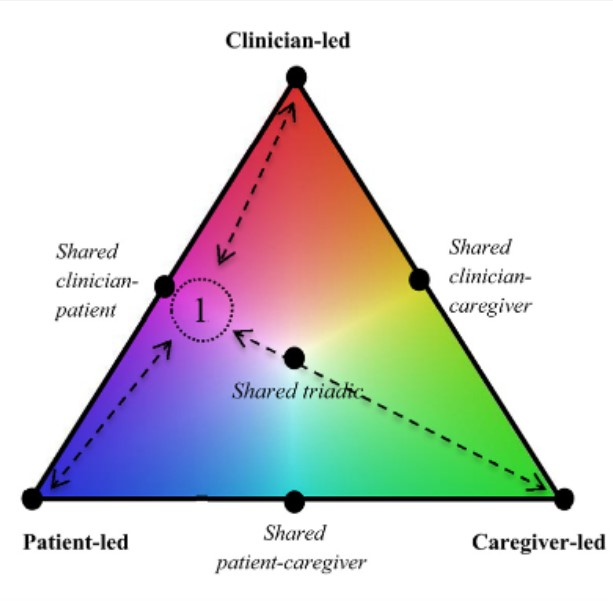
\includegraphics[width=1\columnwidth]{figures/Triangle1Screenshot.jpg}
  \caption{Focus between the patient and the clinician}
  \label{a:PatientClinician}
\end{subfigure}%
\hfill
\begin{subfigure}{.45\columnwidth}
  \centering
  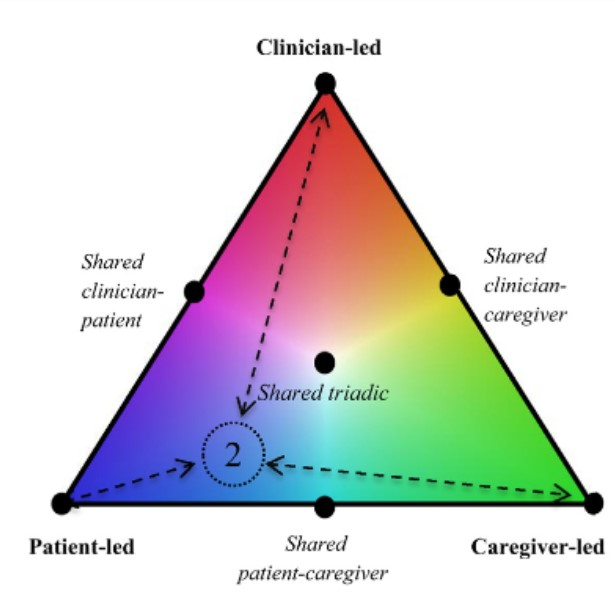
\includegraphics[width=1\columnwidth]{figures/Triangle2Screenshotjpg.jpg}
  \caption{Focus between the patient and the carer}
  \label{b:PatientCarer}
\end{subfigure}
\caption{TRIO Framework/Triangle. Figures from}
\label{fig:TRIO Framework/Triangle}
\end{figure}

% double figure stops here

A third case is where a patient with limited English proficiency has cancer and his son, fluent in English, exchanges all information with the oncologist. The son directs the conversation with consent of the patient. The decision-making focus relies on the son, the caregiver.

Knowing how much each party is involved is important for TRIO’s e-learning platform as all three are target groups for the website. Triadic communication has been shown to be helpful in medical encounters but can also be challenging \cite{Laidsaar-Powell2013}. To facilitate this, psychologists, clinician experts and academics have through years of research determined the TRIO guidelines. These have been used to design the TRIO e-learning modules. Guidelines consist of enhancing the collaboration of caregivers' involvement in medical encounters of oncology as well as how to handle challenging interactions with caregivers \cite{Laidsaar-Powell2018a, Laidsaar-Powell2018}.

What roles family members have in the decision-making of treatment for people with chronic diseases has been studied by Lamore, K. et al. ~\cite{Lamore2017}. Family members need to be provided with medical knowledge and often want to participate in decision-making discussions. For this, they must have helpful behaviours, not being dominating, providing information and support the patient. The patient must also decide when they need a private conversation with the physician. This study mentions that all three parties are positive towards the involvement of caregivers in medical consultations and decisions. Although, for this to work well caregivers need information, both medical and behavioural. The TRIO website aims to provide this information, which is why it is important to study the platform before being released for an optimal learning and caregiver involvement. 

How the partner’s involvement is related to decision-making in triadic cancer consultations has been studied by Bracher, M. ~\cite{Bracher2019}. In these consultations the partner has had different roles, behaviours and relationships with the patient and physician. Some have been dominant, interruptive, refusing to cede while other characteristics have been emotional support, helpful contributions such as self-initiated questions. Spouses and children to the patient are more likely to engage than relatives and friends. Some physicians interacted more with the patient than the partner and often shift back the conversation to the patient. This showed how all involved in triadic consultations need to get a better understanding of their role and communication with each other.

A review of research on the health of the caregiver and the patient by Hodges, L. J. et al. ~\cite{Hodges2005} showed there is an association between their well-being. The caregiver’s psychological health and stress level is strongly related to the partner’s health and stress. The patient is very likely to become distressed when their carer does, they then become a similar level of distress. Bevans, M. et al. ~\cite{Bevans2012} have studied how a caregiver’s life and health get influenced by the care-giving responsibilities of a cancer patient. These responsibilities bring stress and burdens that affect the caregiver negatively. Stressful moments are inevitable, but they can be eased. Avoiding barriers between caregivers and physicians by letting caregivers participate in the medical proceedings, is a good prevention. McCarthy, B. ~\cite{McCarthy2011} has studied carers’ information needs. They need information and often want to hear it from the physicians. Often, they have to actively seek it from physicians and can feel ignored. Cases where carers are content with the communication had met their informational needs. This shows how communication is important for everyone’s well-being. The TRIO website has an important aim to fix these issues.  

\subsection{E-learning platforms and their usability}

Ruiz, J. G. et al. ~\cite{Ruiz2006} have studied e-learnings’ effectiveness and how it fits into the medical world. E-learning enhances individual’s individual learning. It can be integrated into education as well as be used during duty hours. Being able to use e-learning in these circumstances, is very convenient for the medical world. The study also points out important things to think about when evaluating an e-learning platform such as the ease of use, navigation, the material, interaction, etc. Without those, the e-learning loses its effectiveness. Therefore, the TRIO e-learning is very suitable for its user groups, if the usability is adequate. 

The first steps in how to develop an e-learning platform for oncologists to improve their information-giving skills has been studied by Stuij S. M. et al. ~\cite{Stuij2018}. They have shown the oncologist’s learning needs within how they should provide information to patients as well as their training preferences within their profession. Oncologist desire to be able to adapt the information for patients, structure the information and deal with patient’s emotions. Focus groups and interviews revealed that the preferred learning method is a digital platform with multimedia content such as videos. Feedback from peers, experts and patients would also be appreciated. They want to be able to adapt their learning to their own personal needs, have it easily accessible and simple of use. The TRIO platform aims to fulfil these needs by letting the user choose which module they want to do without having to follow a particular order, and can complete them whenever they want to. 

Huang, C. ~\cite{Huang2005} shows that designing an interactive multimedia learning tool gives it dynamic content interactive with, which makes learning an active process. Other features to enhance this, is to be able to immediately test your knowledge and easily visualise information. Several steps are recommended to create such a tool. It is needed to understand the learning goal and the user needs to then design the content and utilize adequate technology. Multimedia materials need to be created with website standards and consider human factors. User tests are then required to be able to evaluate and improve the design. Recommended questions to think of are:

\begin{itemize}
    \item what they will learn, 
    \item why would they want to learn this, 
    \item what they can do on the page and get feedback on how they are doing. 
\end{itemize}

When the module is built, user tests and heuristic evaluation are needed to know how the modules perform. Technical problems can interfere with the learning outcome. Science, education and technology knowledge must be combined for an excellent educational media. The current state of the TRIO website is that it needs to be evaluated to get its best user experience which will be reported in this study. 

\subsection{Purpose and research question}
The TRIO e-learning platform aims to enhance the communication between all parts of the TRIO framework. This is an important objective for the well-being of patients, carers and clinicians. To achieve this the usability of the e-learning must be adequate. To achieve this, this study aimed to answer the following research question; What are the strengths and weaknesses of the TRIO interfaces for clinicians, carers and patients in terms of their usability?

\section{Method}
This section describes the scientific methodology used to answer the research question. The method includes analysing and conducting think-alouds, heuristic evaluation and time logs.

To discover major usability flaws, a heuristic evaluation has been conducted. The problems found have been ranked according to their severity, prevalence and ease to solve. Severity is ranked from 1-5 where 1 is the most severe and 5 the least severe in terms of usability and stopping the user to use the functions properly. Prevalence is ranked from 1-5 where 1 is not a frequently occurring problem and 5 is a frequently occurring problem. The ease to solve is ranked from 1-5 where 1 is a hard and time consuming problem to fix and 5 is an easy problem to fix, less time consuming. 

Think-alouds have several advantages as described by J. Nielsen \cite{nielsen2012thinking} such as being simple to learn. This is beneficial for the collaboration with the TRIO team and the participants that are not familiar with this method. The think-alouds have been conducted remotely with the video-conferencing tool \textit{Zoom} \footnote{https://zoom.us/}. This has enabled to record the users' interactions on their screen and hear their comments which is an advantage to analyse the collected data \cite{hammontree1994remote}. All participants have agreed to participate and be kept anonymous.

The used method measures the effectiveness and efficiency of the TRIO e-learning interface as well as its user satisfaction which is three important points that Brooke, J. mentions to analyse the usability of a website \cite{brooke1996sus}.

To determine the e-learning's effectiveness, 8 think-alouds have been conducted remotely with one participant at a time. The conditions for participants to participate were that they are clinicians or nurses, are a patient diagnosed with cancer at least 6 months ago or is a carer to such a patient. Four think-alouds were with clinicians and nurses, two with carers and two with patients.

First, each participant has filled out a questionnaire about their background. During the think-aloud, they got to perform the same tasks that consist of going through several parts of the module that include videos, text and various interactions. After this, to determine the user satisfaction, the participants were welcomed to give free comments about their experience interacting with the e-learning module. Lastly, the users got to fill out a System Usability Score (SUS) questionnaire \cite{brooke1996sus}. The SUS questionnaire contains 10 questions to which the participants answered with a 5 responses scale from strongly disagree to strongly agree. This determines if the website is usable or not \cite{brooke1996sus}.

The time spent to complete the modules has been logged to determine the efficiency of the e-learning. 

To analyse the collected data, the think-alouds have been transcribed and important usability aspects highlighted. 

\section{Results}
\raggedbottom

\subsection{Heuristic evaluation}
Using heuristic evaluation, 44 problems were found. The usability problems found are presented in this section. Less severe problems that are not presented here are some content problems such as spelling mistakes or inconsistencies in the use of terms. 

The areas of the identified problems are the following:

\begin{itemize}[noitemsep]
    \item Inconsistency of icons.
    \item Redundancy in buttons.
    \item Buttons and interactions not working.
    \item Responsive design problems in layout on smaller and bigger screens.
    \item Presentation of content.
\end{itemize}

As shown in Table \ref{tab:icons}, 2 problems were identified within the inconsistency of icons. All issues have been classified as easy to solve with the rating 5. They have been classified as severe with the rating 2 and have a prevalence that vary from 1 to 5. 

\begin{table}[H]
    \centering
    \begin{tabular}{|m{6.5cm}|c|c|c|}
    \hline
        \textbf{Problem} & \textbf{S} & \textbf{P} & \textbf{E}\\
    \hline
         Inconsistent use of icons, a star and a book to bookmark  & 2 & 5 & 5\\
    \hline
         Search magnifying glass icon to view content & 2 & 1 & 5\\
    \hline
    \end{tabular}
    \caption{Problems found within inconsistency of icons. S: Severity, P: Prevalence, E: Ease to solve.}
    \label{tab:icons}
\end{table}

As shown in Table \ref{tab:redundancy}, 3 problems were identified within the redundancy of buttons. All issues have been classified as easy to solve with the rating 5. Their severities vary from 1 to 4 and have a prevalence from 1 to 5.

\begin{table}[H]
    \centering
    \begin{tabular}{|m{6.5cm}|c|c|c|}
    \hline
        \textbf{Problem} & \textbf{S} & \textbf{P} & \textbf{E}\\
    \hline
         Can view content through clicking on title and on search icon & 4 & 1 & 5\\
    \hline
         Arrows and back/next buttons have the same function & 2 & 1 & 5\\
    \hline
         When clicking on small play button of videos, big play button stays on screen & 1 & 5 & 3\\
    \hline
    \end{tabular}
    \caption{Problems found within redundancy in buttons. S: Severity, P: Prevalence, E: Ease to solve.}
    \label{tab:redundancy}
\end{table}

As shown in Table \ref{tab:interactions}, 17 problems were identified within buttons and interactions. All issues have been classified with an ease to solve that vary from 3 to 5. Their severities vary from 1 to 4 and have a prevalence from 1 to 5.

\begin{table}[H]
    \centering
    \begin{tabular}{|m{6.5cm}|c|c|c|}
    \hline
        \textbf{Problem} & \textbf{S} & \textbf{P} & \textbf{E}\\
    \hline
         Star when bookmarked goes from green to purple, when unbookmarked does not go back to green  & 4 & 5 & 3\\
    \hline
         "Delete content" is misleading as you want to delete page from bookmarks and not delete the content & 3 & 1 & 5\\
    \hline
         Hover text says "sort", does not explain you should click and drag to place where you want it. "Sort" misleads to think to be able to sort by different categories not manually. & 3 & 1 & 4\\
    \hline
         Top bar with "Title" should not have dots as you cannot move that part & 3 & 1 & 5\\
    \hline
         Not possible to click on whole bar to open it and no highlighted hover feedback when mouse is over the health professional button & 3 & 3 & 3\\
    \hline
         Nothing happens when clicking on the print button* & 1 & 5 & 3\\
    \hline
         Clicking on complete on last page of any part makes the whole dashboard go green although several parts are not completed (but still say "Begin")* & 1 & 5 & 3\\
    \hline
         What is written in textbox does not get saved* & 1 & 4 & 3\\
    \hline
         No error message more than an exclamation mark when textboxes are not filled in & 2 & 5 & 5\\
    \hline
         Can be unclear what the button "save and exit" means & 2 & 5 & 4\\
    \hline
         Not possible to save on what page in a part the user stopped & 1 & 5 & 3\\
    \hline
         Activity progress is lost when clicking on "Save and exit" or when reloading the page & 2 & 4 & 3\\
    \hline
         Clicking to continue a part on Dashboard does not lead to the last visited page in that part & 1 & 5 & 3\\
    \hline
         Clicking on button of video activity gives no feedback & 3 & 4 & 4\\
    \hline
         Nothing happens in card activity* & 1 & 1 & 3\\
    \hline
         Text in textboxes not saved when going back & 2 & 2 & 3\\
    \hline
         No hover highlighted feedback on bubbles to click on & 3 & 2 & 4\\
    \hline
    \end{tabular}
    \caption{Problems found within buttons and interactions. S: Severity, P: Prevalence, E: Ease to solve.}
    \label{tab:interactions}
\end{table}

As shown in Table \ref{tab:responsiveDesign}, 6 problems were identified within the responsive design. All issues have been classified with an ease to solve varying from 3 to 5. Their severities vary from 1 to 4 and have a prevalence from 2 to 5.

\begin{table}[H]
    \centering
    \begin{tabular}{|m{6.5cm}|c|c|c|}
    \hline
        \textbf{Problem} & \textbf{S} & \textbf{P} & \textbf{E}\\
    \hline
         Constant hamburger menus on left and right side, even on big screens & 3 & 5 & 3\\
    \hline
         Text is not aligned with the textbox/bar, text is overlapping each other when opening several information boxes & 1 & 4 & 3\\
    \hline
         "Save and exit" button is only on the first page of each part* & 1 & 5 & 4\\
    \hline
         Guidelines on Dashboard look like divided into two on smaller screens & 2 & 5 & 3\\
    \hline
         No margin on left side of the text on pages, text is almost cut on bigger screens & 2 & 5 & 3\\
    \hline
         No link on guidelines that are referred & 4 & 2 & 5\\
    \hline
    \end{tabular}
    \caption{Problems found within responsive design problems in layout on smaller and bigger screens. S: Severity, P: Prevalence, E: Ease to solve.}
    \label{tab:responsiveDesign}
\end{table}

As shown in Table \ref{tab:content}, 9 problems were identified within the redundancy of buttons. All issues have been classified with an ease to solve varying from 2 to 5. Their severities vary from 1 to 4 and have a prevalence from 1 to 5.

\begin{table}[H]
    \centering
    \begin{tabular}{|m{6.5cm}|c|c|c|}
    \hline
        \textbf{Problem} & \textbf{S} & \textbf{P} & \textbf{E}\\
    \hline
         Unnecessary fading in of text & 3 & 5 & 5\\
    \hline
         Progress bar at bottom of the page, easily unseen, not clear what each section represents & 4 & 5 & 4\\
    \hline
         "EST ~5min" on progress bar - message might not be understood & 4 & 5 & 4\\
    \hline
         Progress bar is not showing the correct progress* & 1 & 5 & 2\\
    \hline
         Some boxes get thinner than others when opened & 2 & 4 & 3\\
    \hline
         No information about the arrow buttons & 1 & 1 & 5\\
    \hline
         Asterisk after names lead to nowhere* & 1 & 5 & 5\\
    \hline
         Choice of green colour on slider for the "bad" part* & 2 & 1 & 4\\
    \hline
         Unclear what you get for completing the training & 3 & 1 & 5\\
    \hline
    \end{tabular}
    \caption{Problems found within presentation of content. S: Severity, P: Prevalence, E: Ease to solve.}
    \label{tab:content}
\end{table}

In total, 37 problems were classified in the tables above. 12 out of 37 problems were seen as easy to solve with the rating 5. 17 out of 37 problems were very prevalent with the rating 5. 12 out of 37 problems were classified as severe with the rating 1. 

Following this evaluation, 8 severe problems were fixed before conducting think-alouds. These are marked with an asterisk "*" in the tables above.

\subsection{Think-alouds}
11 think-alouds have been conducted. The participants were between the age of 35 to 77. XX were computer literate and xx had less computer literacy. XX participants have experience in medical knowledge. 

\subsection{Carers}

\subsection{Interface}
\subsubsection{Strengths}
Two out of two carers have expressed appreciation towards the dashboard. Several aspects of the dashboards are appreciated such as its layout, design and functionalities as stated in the following quote.  

\textit{“I’m really impressed by the dashboard, I like the colours and it looks clear to me where you start and where you finish. It’s really good to have the approximate time for each module and I think that was good.”}

Both carers value the feature to be able to see how much time each part will take, it helps them to plan how to go through the different parts. They also appreciate the modules changing colours depending on if the module has been started or not.

All two carers have chosen to start with the introduction although they are free to start anywhere. Like mentioned below, they like being able to choose how much time to spend on each slide and being free on completing the module in their own pace. 

\textit{“I think it’s handy you’re not obligated to do the whole thing in one go.”} 

\textit{“For me it’s really a benefit that I don't have to sit and wait for somebody else to decide how long the slides are going to take me.”}

Both carers commented on finding the overall navigation of the website and modules easy.

\textit{“I think it’s pretty easy and straightforward. I think anybody who’s used to doing online training, modules and so on will probably find it really easy.”}

They also commented on videos being good and exciting, they like that they are not too long. 

\textit{“I think really the use of videos is so important now. People are expecting to be able to click on stuff so yeah I think that’s great.”}

The interaction to build your own question list and download it with suggested questions you would like to ask is appreciated by one of the carers. 

\textit{“I just think it is useful those websites that have lots of questions. So I can build a question list. Ok I think this is useful.”} 

The interaction of popping bubbles to reveal more information, has shown to been appreciated by a carer.

Including references attracts a carers curiosity and mentions below it is good to have.

\textit{“I’m just gonna click on the references and yeah that’s good you’ve got those.”}

\subsubsection{Areas for improvement}
Two out of two carers mention the redundancy of having both arrows and a next button to get to the next page. They mention the non-intuitiveness of which one to use and to know if these actually have the same function or not. They also mention the downside of the arrows, situated in the middle of the page, the user might not scroll until the end before navigating to the next slide. One carer did not see the next button at first as it is located at the end of the page.

\textit{“I always wonder with these things if the next button and the right arrow do the same job. So I’m just going to ignore the arrows and just use the next button.“}

\textit{“I could easily just press next and I would then miss the most important thing.”}

When opening a definition of the roles of healthcare teams, a carer mentions their expectations of the previous one to close automatically. This interaction has also been shown to not show up properly, text is overlapping, the sizes of the boxes are changing, and one carer seems to be confused about this. The carer sees the problem of the interaction but believes it is still a useful page.

\textit{“This oncologist one has overlapped with the surgeon one. And why is his box so big? Was it like this when the page first came up, I can’t remember?”}

Pages with bullet points have different text sizes between one bullet point and the indented ones. Some words have problems with letters being too close to each other. Both carers mention it is not an appealing feature for the users.

\textit{“It’s almost like it’s different fonts there and there, although it might just be a different text size. On this slide I prefer all being the same.”}

Some text on the pages are fading in which makes it appear slightly after other content and makes the user focus on the other content first, as one of the carer mentions.

\textit{“The three points come up slightly after the italics and I think you probably want the person to be looking at the dot points and then the italics.”}

In the “continue” mode of modules there is a tick exactly like when it says “done”, this is confusing for the user, as the carer states below. 

\textit{“I confused continue with completed because it had a tick. I just visually thought I had finished it.”}

The back and next buttons also show up on the first page of each part. The back button on the first page does nothing which confuses the user, as one carer commented here.

\textit{“I was clicking the back arrow and it wouldn't take me back to the start so.”}

A carer mentions when a video shows up it should be possible to go to the previous ones as the e-learning allows you to complete the module in any order.

\subsubsection{Other notable features}
A carer acknowledges an advantage of being able to bookmark pages. Although, during the think-alouds no carer has used this function. 

\textit{“Oh! So I can bookmark my pages. So this means even when I’ve done the module, if I can’t remember everything I can read it again at a later stage so that might be handy.”}

The colours chosen on the website has been appreciated by one carer but another was unsure if the colours are matching. 

The page explaining icons is appreciated by the carer but this could come earlier in the introduction part as the carer is confused by the icons before coming to that page.

\textit{“You haven’t sort of said what the green star and I guess that’s a printer, but the green star is oh that’s up there to bookmark.”}

After videos there sometimes is activities where the user can write free text to reflect. A carer does not understand the purpose of this activity. 

\subsection{Teaching content}
\subsubsection{Strengths}
Two out of two carers mention they like content emphasising the importance of their role. This has been appreciated in forms of text, quotes and videos. It is a good first knowledge, especially to understand the rest of the module, according to a carer.

\textit{“I think the importance of carers like their role, you know I mean some people may not know what they should and shouldn't do in order to help the person, is good first knowledge. And then I think that would make the other parts very productive for them.”}

The carers agree and can relate to the content. For example, learning about the healthcare system can be overwhelming and one carer mentions to agree with that. Even with background in the health system there are things to learn within healthcare.

Both carers relate to the content about the importance of introducing the carer to health professionals and believes it is useful information. They think slides are very useful especially when it explains something they have experienced.

\textit{“I think this is a very useful slide. When we went in to our first meeting we were just there me and my son did this.”}

The website contains links to a relevant podcast and app which has shown to get interest of one carer. One carer also shows appreciation on starting the module with a welcoming phrase.

Bolding important words takes the attention of a carer to what is important. Using other colours than black or italics is not appreciated, a carer mentions their preference in bolding or putting important information in a box.

\subsubsection{Areas for improvement}
In the definitions of the roles of the healthcare teams some improvements can be made. As expressed in the following quote, some definitions need to be elaborated and not repeat a similar word to the word that is being defined.

\textit{“This cancer care coordinator saying that it coordinates care, it is sort of repeating that. I would simplify and elaborate this sentence about coordinating care.”}

A carer mentions inconsistency when a website link is referred as something specific to a state, but it is a link for the whole country. For the website to be used throughout Australia, it should include all states, mentions a carer. 

\textit{“You’ve got “cancer council NSW” here but if I’m looking at the website address, it looks like the national address, so maybe just remove this NSW here.”}

Some spelling or spacing mistakes have been found by carers and should be avoided.

The e-learning is constituted of a module for each user groups. These modules are constituted of several sections or parts. Both terms are used throughout the module for the same things which inconsistent like the carer mentions. There are other term inconsistencies for example between cancer patient or loved one.

A carer mentions inconsistency in the use of some terms. These are, for example, the use of both sections and parts as well as the use of cancer patient and a loved one. Some terms could have religious connotations which a carer mentions.

A carer also mentions busy slides is not optimal.

\textit{“I think you are making this page very busy with text and it’s a bit confrontational.”}

\subsubsection{Other notable features}
A carer mentions they do not like the used term “carer”, between the terms “support person”, “family member” and “partner” they would prefer the term “advocate”. On the other hand, another carer believes the term “carer” is the more accurate and is unsure if advocating is a word everyone would understand.

The carer module often refers to the carer in the third person, but a carer mentions it would be better to address the content directly to the user by using “you”, especially if the term “carer” is ambiguous. 

A carer has both enjoyed pictures but also questioned some about what they would mean.

\textit{“What’s going on with that picture, why have you chosen that?”}

\textit{“I like that photograph, I think it’s really good.”}

A carer mentions the content has the right level of difficulty and the content is useful. 

\textit{“I find it easy and I’m impressed with the content. I’m glad it’s not too basic, it’s got useful information in there.”}

Although, another carer mentions it can get complex.

\textit{“It’s gone from really simple to quite complex.”}

\subsection{Clinicians}

\subsection{Interface}

\subsubsection{Strengths}
3 out 5 clinicians have mentioned liking the layout of the dashboard as well as the estimated time to complete the different parts. Although, one clinician mentions they find it odd that the time is so precise.

\textit{“5 min that’s ok, I’ve got time at the moment.”}

\textit{“But the time in the top right corner here, is that like how long it should take you to complete that module? It’s very precise, isn’t it?”}

Interactive activities are appreciated by all 5 out of 5 clinicians, both the activities themselves but also the content presented in these activities. For example, the activity of sorting answers into the right category as well clicking on a button when something specific happens in the video. A clinician also mentions they would remember information better when they get challenged in an activity rather than in reading plain text. Having bullet points makes it easier to read, mentions a clinician.

\textit{“I definitely think I find it easier when things are bulleted like short sentences and bullets, that I think it’s making it easier to read.”}

The activities were given a lot of positive feedback in general.

\textit{“Ok, this is good I actually get to do something interactive.”} 

\textit{“The activities were good and it was good to have like a mixture of different activities in there as well. You definitely engage like thousand percent more with the activities”}

\textit{“I think it's good to have that interaction rather than just reading, you know like next slide and that gets a bit boring.”}

\textit{“I think it’s nice to have a few interactive things throughout, I think it breaks up when you are just reading and reading things all the time. I like to have scenarios because otherwise it does get monotonous.”}

A clinician mentions the originality of e.g. the activity of the video with a button to click when something specific happens.

\textit{“Oh it’s pretty good. So that comes up on every time that I’ve clicked on it. I like this section it’s really good. I like that activity. I’ve never done one of those before that’s really good.“}

A clinician likes the activity of writing after watching videos.

\textit{“I think that’s quite good because at least you are giving people a little bit more of themselves, like they can write free text instead of just clicking on things. That you ask people to actually write something is good.”}

3 out of 5 clinicians mention the navigation is easy.

\textit{“The navigation is not a problem“ “that was pretty straightforward.”}

A clinician mentions how important it is for them not having to complete everything in one go.

\textit{“I think that’s really important because you do get caught away and the phone is ringing and you don’t want to have to go back and start over.”}

The topics of the module cover all important things a clinician could think of.

\textit{“Just looking at the other topics here it seems to be quite a variety, seems to cover a lot.”}

\subsubsection{Areas for improvement}
2 out 5 clinicians showed to be confused about the functionality of the "Save and exit" button.

\textit{“How do I get back to the other screen? Save and exit. Oh really?”}

The arrows have not the functions a clinician would have expected.

\textit{“Now this is not doing what I thought it was going to do.”}

A clinician mentions nothing happens when clicking on the bookmarking star. However, they understand it should be a working button.

\textit{“I think this star means to click on it but nothing happens.”}

2 out of 5 clinicians, using the sliders, mention that they can not drag the marker to exact wished position. It is not so intuitive to understand that the marker should be placed only on specific lines. They also mention it works fine ones they have understood how to use it.

\textit{“Do I slide this? Oh! Oh I see it has to sit on one of the white lines. I was kind of looking to slide it anywhere on this bit but it had to go on one of the white lines.”}

\textit{“Let’s see if you can just click and drag hopefully. Ah so just on the lines ok. I think it would be nicer if you could move it wherever you wanted.”}

\textit{“Ok it gets a bit easier as you go.”}

2 out of 5 clinicians mention the text size is small and would not mind having it bigger or being able to change it.

\textit{“The font size, I’m leaning forward. Yes, can I change it actually?”}

\textit{“My laptop, it makes text a little bit smaller.”}

A clinician, that can not see the whole page on their screen, wonders what part of the screen is the important one for the video with a button activity.

\textit{“Do I need more of the top page or the bottom page?”}

\subsubsection{other notable features}
A clinician mentions the colours of pages. They prefer to read text on a non-white background, it feels less harsh they state.

\textit{“It’s slightly hard to read and I think it’s something about the white and black backgrounds actually. This is quite harsh and I don’t know if it’s just my eyes but I’m actually finding that a bit harder to focus on than with the slightly coloured background.”}

The meaning of bubbles seems to confuse a clinician. While 2 others find it is easy to read and attracts their attention.

\textit{“I’m not sure why there are 3 bubbles here.”}

\textit{“I’m finding this blurb a bit more easier to read but I don’t know if it’s just that it attracts my interest more. But I think maybe because there are examples in there and that helps.”}

\textit{“See this makes me wanna click on it which is what you want us to do yeah. I like the bubbles! Yeah I quite like that.”}

In the video activity with a button, two clinicians mention it is not clear how many times to click. Some like the activity anyway but it pushes off another clinician of liking this activity.

\textit{“Does that really count or should I click anyway? It was a bit hard when I was doing it, it was a bit hard to know at which point to click.”}

\textit{“Did I press enough for this one? Oh it’s every time I pressed. I only got 6 out of 12. Sometimes he was just going on with the same thing, so I didn’t want to overpress. Ok so how do I feel about pressing every time, I’m not sure about that. I wasn’t that comfortable with that.“}

\subsection{Teaching content}
\subsubsection{Strengths}
5 out of 5 clinicians mention they like content, both written and in video, that they can relate to. They find many important topics in the content. 

\textit{“This is very relevant, in particular to my current patients. Sorts of remind me why I take time to interview patients and relatives separately then bring them together.”}

\textit{“It's definitely something that we deal with a lot day to day. And I think it’s taken my attention because I think understanding these things more definitely has a direct impact day to day on what we do.”}

\textit{“This is really important, that’s what I kind of do all the time.”}

\textit{“That’s interesting the bit about confidentiality. I do worry about that sometimes. Sometimes not sure what the boundaries are.”}

3 out 5 clinicians comment on appreciating videos both for being different from text but also for its quality in content and acting.

\textit{“I think that’s good. I think listening to her language, I think that’s what I struggle with. A lot of the struggle is how to choose the right words to say what she said. So she’s done that very eloquently and it’s good to hear that point.”}

\textit{“Oh a video that’s interesting, it’s sort of mixing it up, it’s nice to have the different things.”}

\textit{“It’s very good how she looked very angry and he is like protecting.”}

\textit{“I totally agree with that comment there. I can relate to that one.”}

A clinician mentions they like scenarios, like in the videos.

\textit{“I like scenarios. Personally I quite like them. Just sort of triggers you to think a little bit more rather than just reading through something like yeah I think the scenario allows me to put it into practice or put it into place a little bit more.”}

A clinician shows curiosity about topics they don’t know about, they want to learn more.

\textit{“Family dominance what does that mean? Makes me wanna click on it so I can find out what it’s all about.“}

2 out of 5 clinicians also mentioned the value of bringing up the importance of carer’s involvement. Facts about it are also good to emphasise on the carer’s needs.

\textit{“Family need to be involved and there is a lot of stress involved so that was good it was pointed out“}

\textit{“You have explanations of why it is important and I agree with all of this.”} 

\textit{“Oh my gosh that’s a lot of unmet needs! So that’s good because that basically just tells you that you need to be really aware that they have all these unmet needs. You can’t assume that they are ok just because they are not the sick one.”}

2 out of 5 clinicians mention they like content that they can skim through, where the important information is quickly understood. A simple but not too basic language is also appreciated. Busy slides is not appealing and they mention they may not retain the important information.

\textit{“You don’t want to make it sound childish because that puts people off and makes them disinterested.”}

\textit{“When I read something apart from patients notes, I skim it. So it’s gotta be something that’s going, that I can get the message with a glance.”}

\textit{“I think to be honest if I was doing this I would probably gloss over things where there’s lots of writing and I would just be going on to ok where is something that I can actually do.”}

\textit{“I mean on that slide you get the principles you just go yeah yeah. This is the kind of slides you pass over a lot more quickly than you get from...than the interactiveness that draws you to engage much more with what’s being written.”}

2 out of 5 clinicians mention they like having references throughout the text.

\textit{“I quite like the way the little references pop up, that’s quite easy to use.”}

3 out 5 clinicians mention the quotes are good and useful.

\textit{“I like the use of the quotes. It gives a bit of a supportive evidence to it, as a nurse I like that.”}

A clinician mentions they like links to other sources, so they know it is a trusted source.

\textit{“It’s good to have that link in, because there are definitely times where you think things from online are abused, so that’s good to know.”}

\subsubsection{Areas for improvement}
It is unclear for a clinician what they would get for completing the module.

\textit{“What do I get in the end of this? A certificate, coffee, voucher, points?”}

Inconsistency of term in using family member, carer and family carer has been mentioned by a clinician.

\textit{“We are gone with the term family carers here. It’s hard isn’t it. Kind of rolled it into one there.”}

A clinician has also found some minor spelling mistakes.

\subsubsection{Other notable features}
A clinician mentions he would probably not download a summary of each part unless there would be new information in it. Although, another clinician believes it is good summaries. It is not clear for a clinician what it does but after trying they like the function.

\textit{“Download summary. Not sure why I would download this summary. If there was more information I probably would. Or a list of other resources.”}

\textit{“I think that’s a quite good summary slide of what’s being said.”}

\textit{“What does the “Download summary” do? Oh so it will open as a PDF? So someone could print it and get a hard copy? Ok that’s good!”}

Two clinicians mentions they would start the module at the beginning and go through it systematically while another mentions they would first do the compulsory parts and then what they are interested in.

\textit{“I would probably do the compulsory ones and then go ok what am I actually interested in.”}

\textit{“Where would you start? Uh the introduction.”}

A clinician does not understand the meaning of certain pictures. 2 out 5 clinicians recognise some pictures from other training they have done.

\textit{“Not sure what that picture was. A building?”}

\textit{“Oh I’ve seen that picture before.”}

\subsection{Patients}

\subsection{Interface}
\subsubsection{Strengths}
A patient finds the navigation and instructions easy and intuitive. Another patient is not able to navigate through the program by their own.

\textit{“Easy enough to navigate. It is quite intuitive.”}

\textit{“Overwhelming, once you get into the thing, I have no idea what I have to do.”}

A patient mentions they like being able to know how much time each part will take.

\textit{“I like the fact that it gives you an idea of how long it is going to take.”}

The function of being able to create a question list and download it, is appreciated by a patient.

\textit{“I like the whole message of the page, this is about how they can prepare a list of questions. You can click on whatever ones that you want, yeah so this is really good. So then you download the checklist. I like that, I like that a lot.”}

The patient likes interactive things like activities. The activity of creating your care team has also shown to be appreciated by 2 out of 3 patients. A patient with struggles to navigate through the website would not like to do this activity.

\textit{“ Some of the activities like the questions, I really liked. The ones where you wrote down what you thought the carer might do for you if you then use it as a communication tool, really good as well.”}

\textit{“I think that’s really good. It sort of covers everything, doesn’t it? So people know that they got a wide sort of section of people that can help.”}

A patient gives positive general feedback about the e-learning.

\textit{“It is a wonderful program for people to understand about all the things that happen when you get cancer and it’s wonderful.”}

\subsubsection{Areas for improvement}
A patient does not know how to interact with the slider. When they figure out how to slide it, it does not work smoothly. This makes that the patient does not enjoy this interaction.

\textit{“So you just click on supporter. It’s not opening. That drag is a bit space. To be honest I don’t like this little thing.”}

\subsubsection{other notable features}
The bubbles are appreciated by a patient. Another patient does not understand how to use the bubbles, they think they shouldn’t click on them because they present myths. A clear instruction is missing for this activity.

\textit{“I like the bubbles.”}

\textit{““- What do you feel like you should do with these? - Not click on any of them! [....] You should just say it, please click on the myth that you… It needs to be explained a bit more I think.”}

\subsection{Teaching content}
\subsubsection{Strengths}
A patient mentions they like pictures to make the text more engaging and pages more appealing. 
\textit{“So instantly more engaging because there is a photo. Visually appealing with this photo.”}

One also mentions finding the text clear and easy to read with a good font. 

\textit{“It is clear and it’s an easy-to-read font.”}

A patient shows interest to the references.

\textit{“Let me jump to your references.”}

2 out of 3 patients enjoy quotes and icons.

\textit{“Immediately better because there is a little icon or something and this quotation. I liked that. Quotation immediately makes it more personable. Lovely really nice. So breaks it up with little quotation.”}

\textit{“Good. Quotes are good. Quotes make it more personal. You know makes you feel that there is empathy there, a bit of empathy I think when you here real stories and that and we like real stories”}

All patients appreciate content about the benefits of having a carer, their importance and roles they can have. 

\textit{“"What are the benefits of supporting", that’s good.”}

\textit{“I get your message about including the family in consultations and a couple of tips and stuff like that. They are the gems.”}

\textit{“If I was caring for someone, I’d wanna know what I can do and couldn't do. And what would be the best thing to do or not to do.”}

\textit{““Family and friends can play a very important role during care” great, that’s a great first line.”}

A patient finds pages visually attractive when there are clear headings, different colours and examples. 2 out 3 patients support highlighted text and would suggest more highlighting.

\textit{“I like the look of this page a lot more. So it’s already more visually attractive. It’s not just, I mean there are sentences but you have given clearer headings. Ok and there are some examples so it’s practical.”}

\textit{“Even with heavy text, the fact that you have highlighted them in different colours immediately makes them more accessible to focus.”}

2 out of 3 patients relate and agree with the content.

\textit{“Does that sort of brings you to your experience? - Yeah. Yeah yeah yeah. ”}

\textit{“That was the main thing, the most important thing that I felt, it was the fear.”}

A patient mentions the content in summaries are important. Another important content mentioned by a patient is the truths of myths.

\textit{“That last summarise there is very important.”}

\textit{“- What we’re trying to do is to challenge those believes that. - Oh that seem very important.”}

\subsubsection{Areas for improvement}
A patient mentions text heavy slides are not appealing and not beneficial for their learning.

\textit{“It is pretty text heavy and I guess that I am more of a visual learner so it might be nice to have some more pictures, icons,  to make it a little bit more visually appealing.”}

A patient would like to see more statistics. 

\textit{“I like statistics, you’ve got 4 pages of references there, I bet that you can throw in some statistics. Some people remember by numbers.”}

A patient finds the text font a bit to big so that it looks like headers and not actual text. Another patient believe the text size is good.

\textit{“Fonts are a tiny bit big so it comes across as a header rather than a textbox.”}

\textit{“- How is the size, font and readability of it? - It’s nice.”}

\subsubsection{Other notable features}
A patient skips all videos because it is not their thing. Another one also mentions they would probably not watch them.

\textit{“I’m not going to play that. I’m not a very video type people.”}

\textit{“I think I’ll probably skip that.”}

A patient mention they would prefer more technical language to get their interest.

\textit{“So because of my background and everything else, so this for me is like super basic super like I wouldn’t keep reading it. But if it had you know perhaps lots of you know reasons why, like statistics or better outcomes or whatever for me a bit more technical language, that would be fine.”}

\subsection{System Usability Score questionnaire}
All participants have answered 10 questions from the System Usability Score questionnaire. The answers are represented in table xx below. 

\section{Discussion}
discuss \\
- comapare HE and TA \\
- good to be free to to in whatever order, some would do it in order and some not \\

\subsection{Method criticism}
Use of Zoom:\\
- participants have not used it before, unable to get screen sharing, unable to make login into the eTrio (interviewer has to click through for participant)\\
- new for interviewer as well, finding new functions like participant can click on interviewer's screen

\subsection{Future research}
On laptops the layout has mostly been display properly. Carers mention that they wonder how it would look like on smaller devices. 

\textit{“Would I be able to read it on my iPhone?”}

\textit{“I’m on my laptop now, not on my phone or my iPad, so I don’t know how it would display on those devices, but on my laptop everything is easy to read.”}

Briz-Ponce, L. ~\cite{Briz-Ponce2017} show that most student participants of the study own a mobile device and that mobile technologies are constantly increasing. Medical students are positive towards mobile learning and would recommend it. However, their willingness of use is only medium high as they had a low ease of use perception of mobile learning. This shows how important it is for a mobile learning platform to provide a good user experience. The TRIO website is available on mobile and should therefore be tested with its users. 

\section{Conclusion}
conclude \\
The outcome has given criterias to improve the e-learning website both usability and content wise. tbc.
 
\section{Acknowledgments}

% BALANCE COLUMNS
\balance{}

% REFERENCES FORMAT
% References must be the same font size as other body text.
\bibliographystyle{SIGCHI-Reference-Format}
\bibliography{MasterThesis}

\end{document}

%%% Local Variables:
%%% mode: latex
%%% TeX-master: t
%%% End:
